\begin{figure}[h!]

  % Define the layers to draw the diagram
  \pgfdeclarelayer{tomgombackground}
  \pgfdeclarelayer{tombackground}
  \pgfsetlayers{tomgombackground,tombackground,main}

  % Define a new shape: page with a folded corner 
  \makeatletter
  \pgfdeclareshape{flippedpage}{
    \inheritsavedanchors[from=rectangle] % this is nearly a rectangle
    \inheritanchorborder[from=rectangle]
    \inheritanchor[from=rectangle]{center}
    \inheritanchor[from=rectangle]{north}
    \inheritanchor[from=rectangle]{south}
    \inheritanchor[from=rectangle]{west}
    \inheritanchor[from=rectangle]{east}
    % ... and possibly more
    \backgroundpath{% this is new
    % store lower left in xa/ya and upper right in xb/yb
    \southwest \pgf@xa=\pgf@x \pgf@ya=\pgf@y
    \northeast \pgf@xb=\pgf@x \pgf@yb=\pgf@y
    % compute corner of ``flipped page''
    \pgf@xc=\pgf@xb \advance\pgf@xc by-5pt % this should be a parameter
    \pgf@yc=\pgf@yb \advance\pgf@yc by-5pt
    % diagonal path of the corner 
    \pgfpathmoveto{\pgfpoint{\pgf@xa}{\pgf@ya}}
    \pgfpathlineto{\pgfpoint{\pgf@xa}{\pgf@yb}}
    \pgfpathlineto{\pgfpoint{\pgf@xc}{\pgf@yb}}
    \pgfpathlineto{\pgfpoint{\pgf@xb}{\pgf@yc}}
    \pgfpathlineto{\pgfpoint{\pgf@xb}{\pgf@ya}}
    \pgfpathclose
    % add little corner
    \pgfpathmoveto{\pgfpoint{\pgf@xc}{\pgf@yb}}
    \pgfpathlineto{\pgfpoint{\pgf@xc}{\pgf@yc}}
    \pgfpathlineto{\pgfpoint{\pgf@xb}{\pgf@yc}}
    \pgfpathlineto{\pgfpoint{\pgf@xc}{\pgf@yc}}
    }
  }

  % Define block styles
  \tikzstyle{compiler}=[draw, fill=blue!20, text width=6em, text centered, minimum height=2.5em, rounded corners]
  \tikzstyle{code}=[draw,shape=flippedpage,text width=2.7em, text centered, minimum height=3.7em,fill=white]
  \tikzstyle{texttitle}=[fill=white, rounded corners, draw=black!50, dashed]
  \tikzstyle{background}=[fill=yellow!20, rounded corners, draw=black!50, dashed]

  \begin{center}
  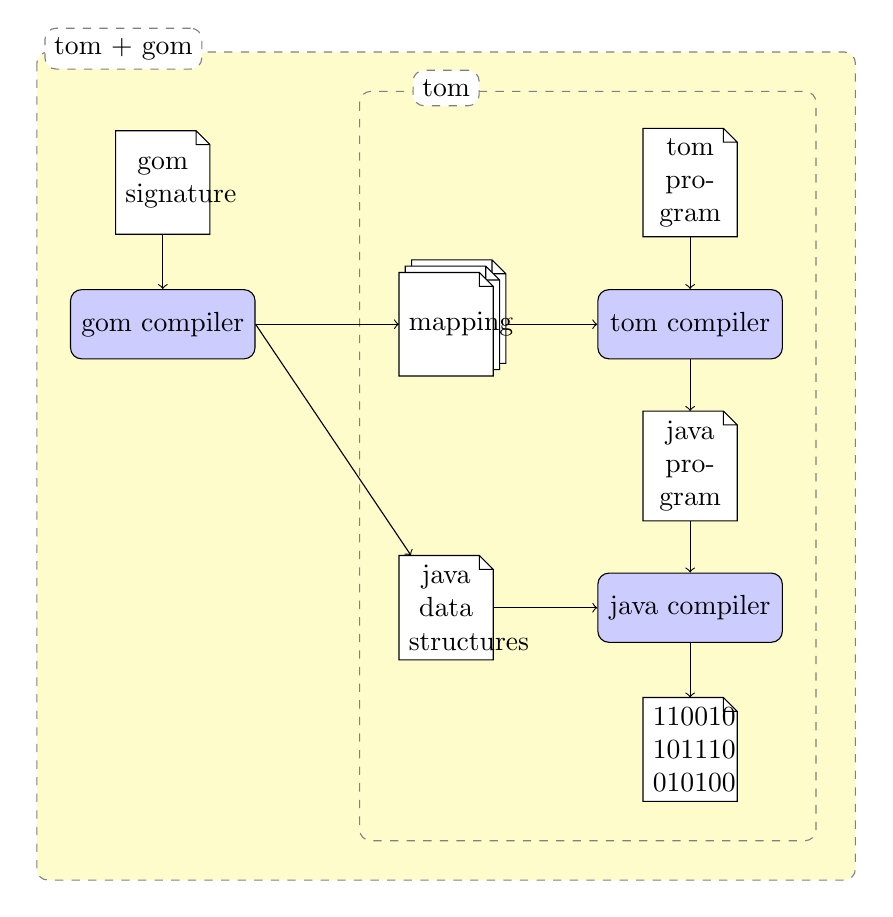
\begin{tikzpicture}
    % Draw diagram elements
    
    % Draw an invisible paper and back papers
    \node (invisiblemapping) [text width=2.7em, minimum height=3.7em] {};
    \path (invisiblemapping)+(0.0,0.16) node (mappingzero) [code] {};
    \path (mappingzero)+(-0.08,-0.08) node (mappingone) [code] {};
    \path (mappingone)+(-0.08,-0.08) node (mapping) [code] {\figcode{mapping}};

    \path (mapping)+(0.0,-3.6) node (datastruct)[code] 
    {\figcode{java data}\\ \figcode{structures}};
    \path (mapping.east)+(2.5,0.0) node (tomcomp)[compiler] 
    {\figcode{tom compiler}};
    \path (mapping.east)+(2.5,1.8) node (tomcode)[code] 
      {\figcode{tom program}};
    \path (mapping.east)+(2.5,-1.8) node (javacode)[code] 
      {\figcode{java program}};
    \path (mapping.east)+(2.5,-3.6) node (javacomp)[compiler] 
      {\figcode{java compiler}};
    \path (mapping.east)+(2.5,-5.4) node (bytecode)[code]
      {\figcode{110010}\\\figcode{101110}\\\figcode{010100}};

    % Draw gom side
    \path (mapping.west)+(-3.0,0.0) node (gomcomp)[compiler] 
    {\figcode{gom compiler}};
    \path (mapping.west)+(-3.0,1.8) node[code] (gomsig) {\figcode{gom} \\ \figcode{signature}};

    % Draw arrows between elements
    \path [draw, ->] (gomsig.south) -- node [left] {} (gomcomp);
    \path [draw, ->] (gomcomp.east) -- node [above] {} (mapping);
    % Use invisible mapping to avoid arrow cover back papers
    \path [draw, ->] (invisiblemapping.east) -- node [above] {} (tomcomp);
    \path [draw, ->] (gomcomp.east) -- node [above] {} (datastruct);
    \path [draw, ->] (datastruct.east) -- node [above] {} (javacomp);
    \path [draw, ->] (tomcode.south) -- node [left] {} (tomcomp);
    \path [draw, ->] (tomcomp.south) -- node [left] {} (javacode);
    \path [draw, ->] (javacode.south) -- node [left] {} (javacomp);
    \path [draw, ->] (javacomp.south) -- node [left] {} (bytecode);

    % Draw layer titles
    \path (gomsig)+(-0.5,1.7) node (tomgomtitle) [texttitle]
      {\code{tom + gom}};
    \path (mapping)+(0.0,3.0) node (tomtitle) [texttitle]
      {\code{tom}};

    % Draw tomgombackground
    \begin{pgfonlayer}{tomgombackground}
      % Left-top corner of the background rectangle
      \path (gomsig.west |- gomsig.north)+(-1.0,1.0) node (a) {};
      % Right-bottom corner of the background rectangle
      \path (bytecode.east|- bytecode.south)+(1.5,-1.0) node (b) {};

      % Draw the background
      \path[background]
      (a) rectangle (b);
    \end{pgfonlayer}

    % Draw tombackground
    \begin{pgfonlayer}{tombackground}
      % Left-top corner of the background rectangle
      \path (mapping.west |- mapping.north)+(-0.5,2.3) node (a) {};
      % Right-bottom corner of the background rectangle
      \path (bytecode.east|- bytecode.south)+(1.0,-0.5) node (b) {};

      % Draw the background
      \path[background]
      (a) rectangle (b);
    \end{pgfonlayer}

  \end{tikzpicture}
  \end{center}
  \caption{Processus de compilation d'un programme {\tom}}
\label{fig:compilation}
\end{figure}

